

\subsection{Use case: Groups}
	\subsubsection{Use case diagram}
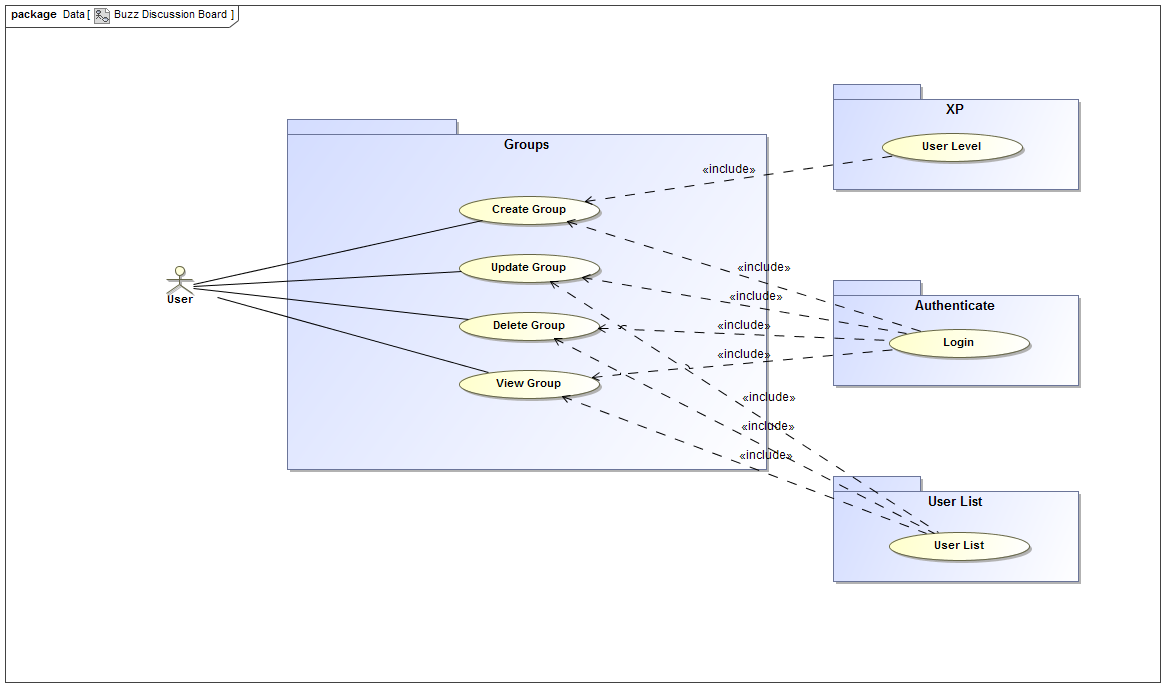
\includegraphics[width=\textwidth]{groups}
	\subsubsection{Short description}
	\begin{description}
		\item When a user want to create/enter a Buzz Space, first he creates a group or are part of the user-list for the group that owns the buzz space he tries to access. 


		\item[] Different actors:
		\begin{itemize}
			\item Administrator.
			\item User.   
		\end{itemize}
		
	\end{description}

	
	\subsection{Use case prioritization}
	\begin{description}
		\item[] Critical
		\begin{itemize}
			\item Create Group
			\item Update Group
			\item View Group
		\end{itemize}
		\item[] Important
		\begin{itemize}
			\item Delete Group
			\item Create Group - Admin
			\item Update Group - Admin
			\item Delete Group	 - Admin		
		\end{itemize}
	\end{description}
	\subsubsection{Use cases}

\newpage
\begin{table}
\begin{tabularx}{\textwidth}{|>{\setlength\hsize{0.7\hsize}\setlength\linewidth{\hsize}}X|>{\setlength\hsize{.8\hsize}\setlength\linewidth{\hsize}}X|>{\setlength\hsize{.8\hsize}\setlength\linewidth{\hsize}}X|>{\setlength\hsize{0.7\hsize}\setlength\linewidth{\hsize}}X|}
\hline
	\multicolumn{4}{|c|}{\textbf{Use cases for Groups}}\\
\hline
	\paragraph{Use Case} & \paragraph{Preconditions} & \paragraph{Post-conditions} & \paragraph{Description} \\
\hline
	\paragraph{Create Group}
&
\begin{itemize}
	\item User is logged in
	\item The group should not exist
	\item Is on XP where group creation is allowed 
\end{itemize} &
\begin{itemize}
	\item Group is created
	\item Group is saved in database
\end{itemize} &
	\paragraph{A logged in user try to create a group. Permission to create a group is dependent on the user's XP} 
	
\\
\hline
	\paragraph{Update Group}
&
\begin{itemize}
	\item User is logged in
	\item The group should exist
	\item Is part of the user-list for that group
	\item Is set to admin for the group in the user-list
\end{itemize} &
\begin{itemize}
	\item Group details is changed
	\item Changes are saved in database
	\item All members of group is notified
\end{itemize} &
	\paragraph{Changes to the group's details can only be made by the admins of the group as set out in the user-list}
\\

\hline

	\paragraph{Delete Group}
&
\begin{itemize}
	\item User is logged in
	\item The group should exist
	\item Is part of the user-list for that group
	\item Is set to admin for the group in the user-list
\end{itemize} &
\begin{itemize}
	\item Group is deleted
	\item Group is marked as deleted in database
	\item All members of group is notified
\end{itemize} &
	\paragraph{Deleting a group can only be done by the admins of the group as set out in the user-list}
\\
\hline

	\paragraph{View Group}
&
\begin{itemize}
	\item The group should exist
	\item The group should be publicly visible	
\end{itemize} &
\begin{itemize}
	\item Group details are accessed
\end{itemize} &
	\paragraph{Anyone can view the group's info if the group is a public group}
\\
\hline
	\paragraph{View Group - Hidden}
&
\begin{itemize}
	\item User is logged in
	\item The group should exist
	\item Is part of the user-list for that group
\end{itemize} &
\begin{itemize}
	\item Group details are accessed
\end{itemize} &
	\paragraph{Anyone in the group's user-list can view the group's info when the group is a hidden group}
\\
\hline


\end{tabularx}
\end{table}

\newpage
\begin{table}
\begin{tabularx}{\textwidth}{|>{\setlength\hsize{0.7\hsize}\setlength\linewidth{\hsize}}X|>{\setlength\hsize{.8\hsize}\setlength\linewidth{\hsize}}X|>{\setlength\hsize{.8\hsize}\setlength\linewidth{\hsize}}X|>{\setlength\hsize{0.7\hsize}\setlength\linewidth{\hsize}}X|}
\hline
	\multicolumn{4}{|c|}{\textbf{Use cases for Groups}}\\
\hline
	\paragraph{Use Case} & \paragraph{Preconditions} & \paragraph{Post-conditions} & \paragraph{Description} \\
	\paragraph{Create Group - Admin}
&
\begin{itemize}
	\item User is logged in as Admin
	\item The group should not exist
\end{itemize} &
\begin{itemize}
	\item Group is created
	\item Group is saved in database
\end{itemize} &
	\paragraph{A logged in Admin can add a group. } 
	
\\
\hline
	\paragraph{Update Group - Admin}
&
\begin{itemize}
	\item User is logged in as Admin
	\item The group should exist
\end{itemize} &
\begin{itemize}
	\item Group details is changed
	\item Changes are saved in database
	\item All members of group is notified
\end{itemize} &
	\paragraph{Changes to the group's details can only be made by the admins of the buzz system}
\\

\hline

	\paragraph{Delete Group - Admin}
&
\begin{itemize}
	\item User is logged in as Admin
	\item The group should exist
\end{itemize} &
\begin{itemize}
	\item Group is deleted
	\item Group is marked as deleted in database
	\item All members of group is notified
\end{itemize} &
	\paragraph{Deleting a group can be done by the admins of the buzz system}
\\
\hline





\end{tabularx}
\end{table}

